\chapter{Continuous-wave lineal frequency modulation (CWLFM) radars for gait analysis}
\chaptermark{CWLFM radars for gait analysis}

It has been shown in \cref{cha:generalities} that the most promising method for gait analysis involves the use of continuous-wave lineal frequency modulation (CWLFM) radars. Employing a single radar or a network of radars to analyse gait and extract useful information has been proved accurate and robust to other factors that could hinder the data extraction from the signals, compared to other methods. For that matter, it has been shown that current radar solutions require voluminous, expensive and inefficient hardware that is not scalable and easy to deploy in real-life scenarios, should the gait of a patient be analysed.

Moreover, the current system proposals are designed exclusively to work with one radar node. State-of-the-art research is now focused on implementations that feature a multi-static radar network, composed of several radar nodes, positioned in different locations that ---by working synchronously--- can extract data simultaneously, and by processing the netted radar signals, the extraction of more accurate and useful information for gait analysis is achieved [REF ZZZ]. The current design described in \cref{cha:generalities} is not suitable for modification to support the configuration of a radar network of multiple nodes. It is of interest to design a new radar system pipeline that can be adapted to work in a multi-static radar network. In this chapter, a new radar node design is described, which addresses the problems of current implementations, focusing on compactness, energy-efficiency, cost-efficiency and ability to be adapted to work in a multi-static radar network.

\section{Radar and communications requirements}

To understand the characteristics of the radar signal used for gait analysis, it is important to fix the radar parameters that enable gait analysis in a particular scenario. For the purposes of this Bachelor's Thesis, and aligned to the common application of CWLFM radars for gait analysis [REF ZZZ], an indoor scenario and a target of a human being is considered.

From this context and following from \cref{eq:fs_final}, it is possible to obtain radar parameters that correspond to this context of operation. In \cref{eq:fs_final}, $R_{\max}$ and $\nu_{r\max}$ are constants that depend on the environment and the case of radar use. In this context of measuring the gait of a person, the environment is indoors and the target is a walking human being. The target linear velocity should be around $\SI{5}{\kilo\meter\per\hour} \approx \SI{1.4}{\meter\per\second}$. The goal is to obtain measurements from moving parts of the body. The fastest moving parts are the arms, which have a maximum radial velocity of around \SI{3}{\meter\per\second}. Therefore, $\nu_{r\max} = 1.4 + 3 = \SI{4.4}{\meter\per\second}$. A margin of error is left to avoid measurement errors from sudden movements of body parts. Thus, $\nu_{r\max} =\SI{5.9}{\meter\per\second}$.

With these constraints, it is possible to obtain the minimum sampling frequencies and the maximum pulse repetition intervals for radars with different bandwidths and working frequencies by solving \cref{eq:fs_final}. A series of examples are shown in \cref{tab:fs_Tc}.

\begin{longtable}{@{}cccc@{}}
	\toprule
	$\mathbf{f_0}$ \textbf{(GHz)}& $\mathbf{W}$ \textbf{(GHz)} & $\mathbf{f_{s\min}} \textbf{(MHz)}$& $\mathbf{T_c}$ \textbf{(\si{\micro\second})} \\* \midrule 
	\endhead
	24.0 & 2.0 & 0.5 & 529.7 \\
	24.0 & 4.0 & 1.0 & 529.7 \\
	24.0 & 5.0 & 1.3 & 529.7 \\
	66.0 & 4.0 & 2.8 & 192.6 \\
	134.0 & 1.0 & 1.4 & 94.9 \\* \bottomrule
	\caption{Sampling frequencies and pulse repetition intervals for different parameters.}
	\label{tab:fs_Tc} 
\end{longtable}
	\change[inline]{no me convence esta tabla, cambiar por un gráfico que relacione los distintos aspectos y resumen de lo que se habla en esta sección (en forma de esquema)}
\subsection{Hardware description of the current CWLFM node developed at GMR}
\subsectionmark{Hardware of current CWLFM node}

In this section, the hardware of the currently used radar node at GMR is described.
\subsubsection{RF board}

The printed circuit board (PCB) of the system which handles the emission and reception of the CWLFM signals contains several elements. First, the PCB contains a pair of patch array antennas printed on the surface of the PCB, one antenna is associated with the signal transmission while the other is related to the reception of the rebound signal from the target. The antennas are connected to a monolithic microwave integrated circuit (MMIC) from Silicon Radar, model TRX-024-046 [REF ZZZ Datasheet MMIC] which provides an output signal for transmission and intermediate frequency (IF) signals after reception. The high-level diagram of the MMIC is shown in \cref{fig:block_mmic}. The VCO bandwith is controlled with pins \textit{d0} to \textit{d3} and the frequency tuning is performed by means the \textit{Vctrl} DC voltage level. An image of the resulting PCB with the antennas and MMIC is shown in \cref{fig:rf_board}. This PCB is fabricated in FR4 dielectric material and is part of the SiRadar EvalKit Easy evaluation kit from Silicon Radar [REF to evalkit DS ZZZ].

\begin{figure}[ht]
	\centering
	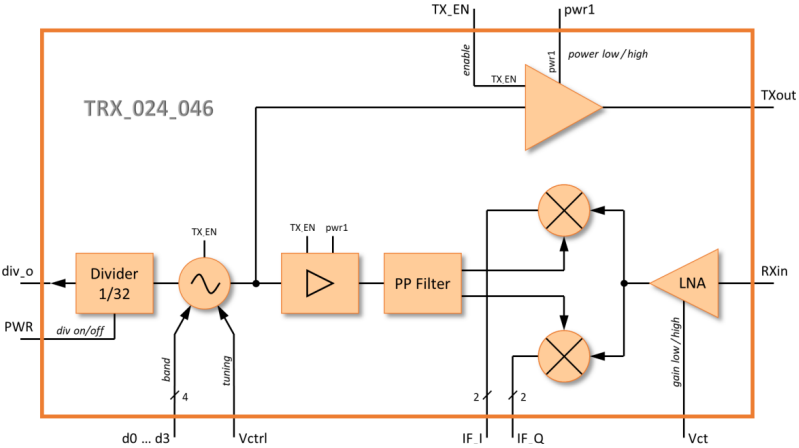
\includegraphics[width=0.8\linewidth]{block_mmic_datasheet.png}
	\caption{High-level diagram of the TRX-024-046 MMIC. The tuning voltage is controlled by the DC level on the \textit{Vctrl} pin and the bandwidth is selected with the \textit{d0...d3} pins. The resulting beating signals are output in the \textit{IF\_I} and \textit{IF\_Q} pins. It is important to note that each pair of IF signals is in differential form \label{fig:block_mmic}}
\end{figure}

\begin{figure}[ht]
	\centering
	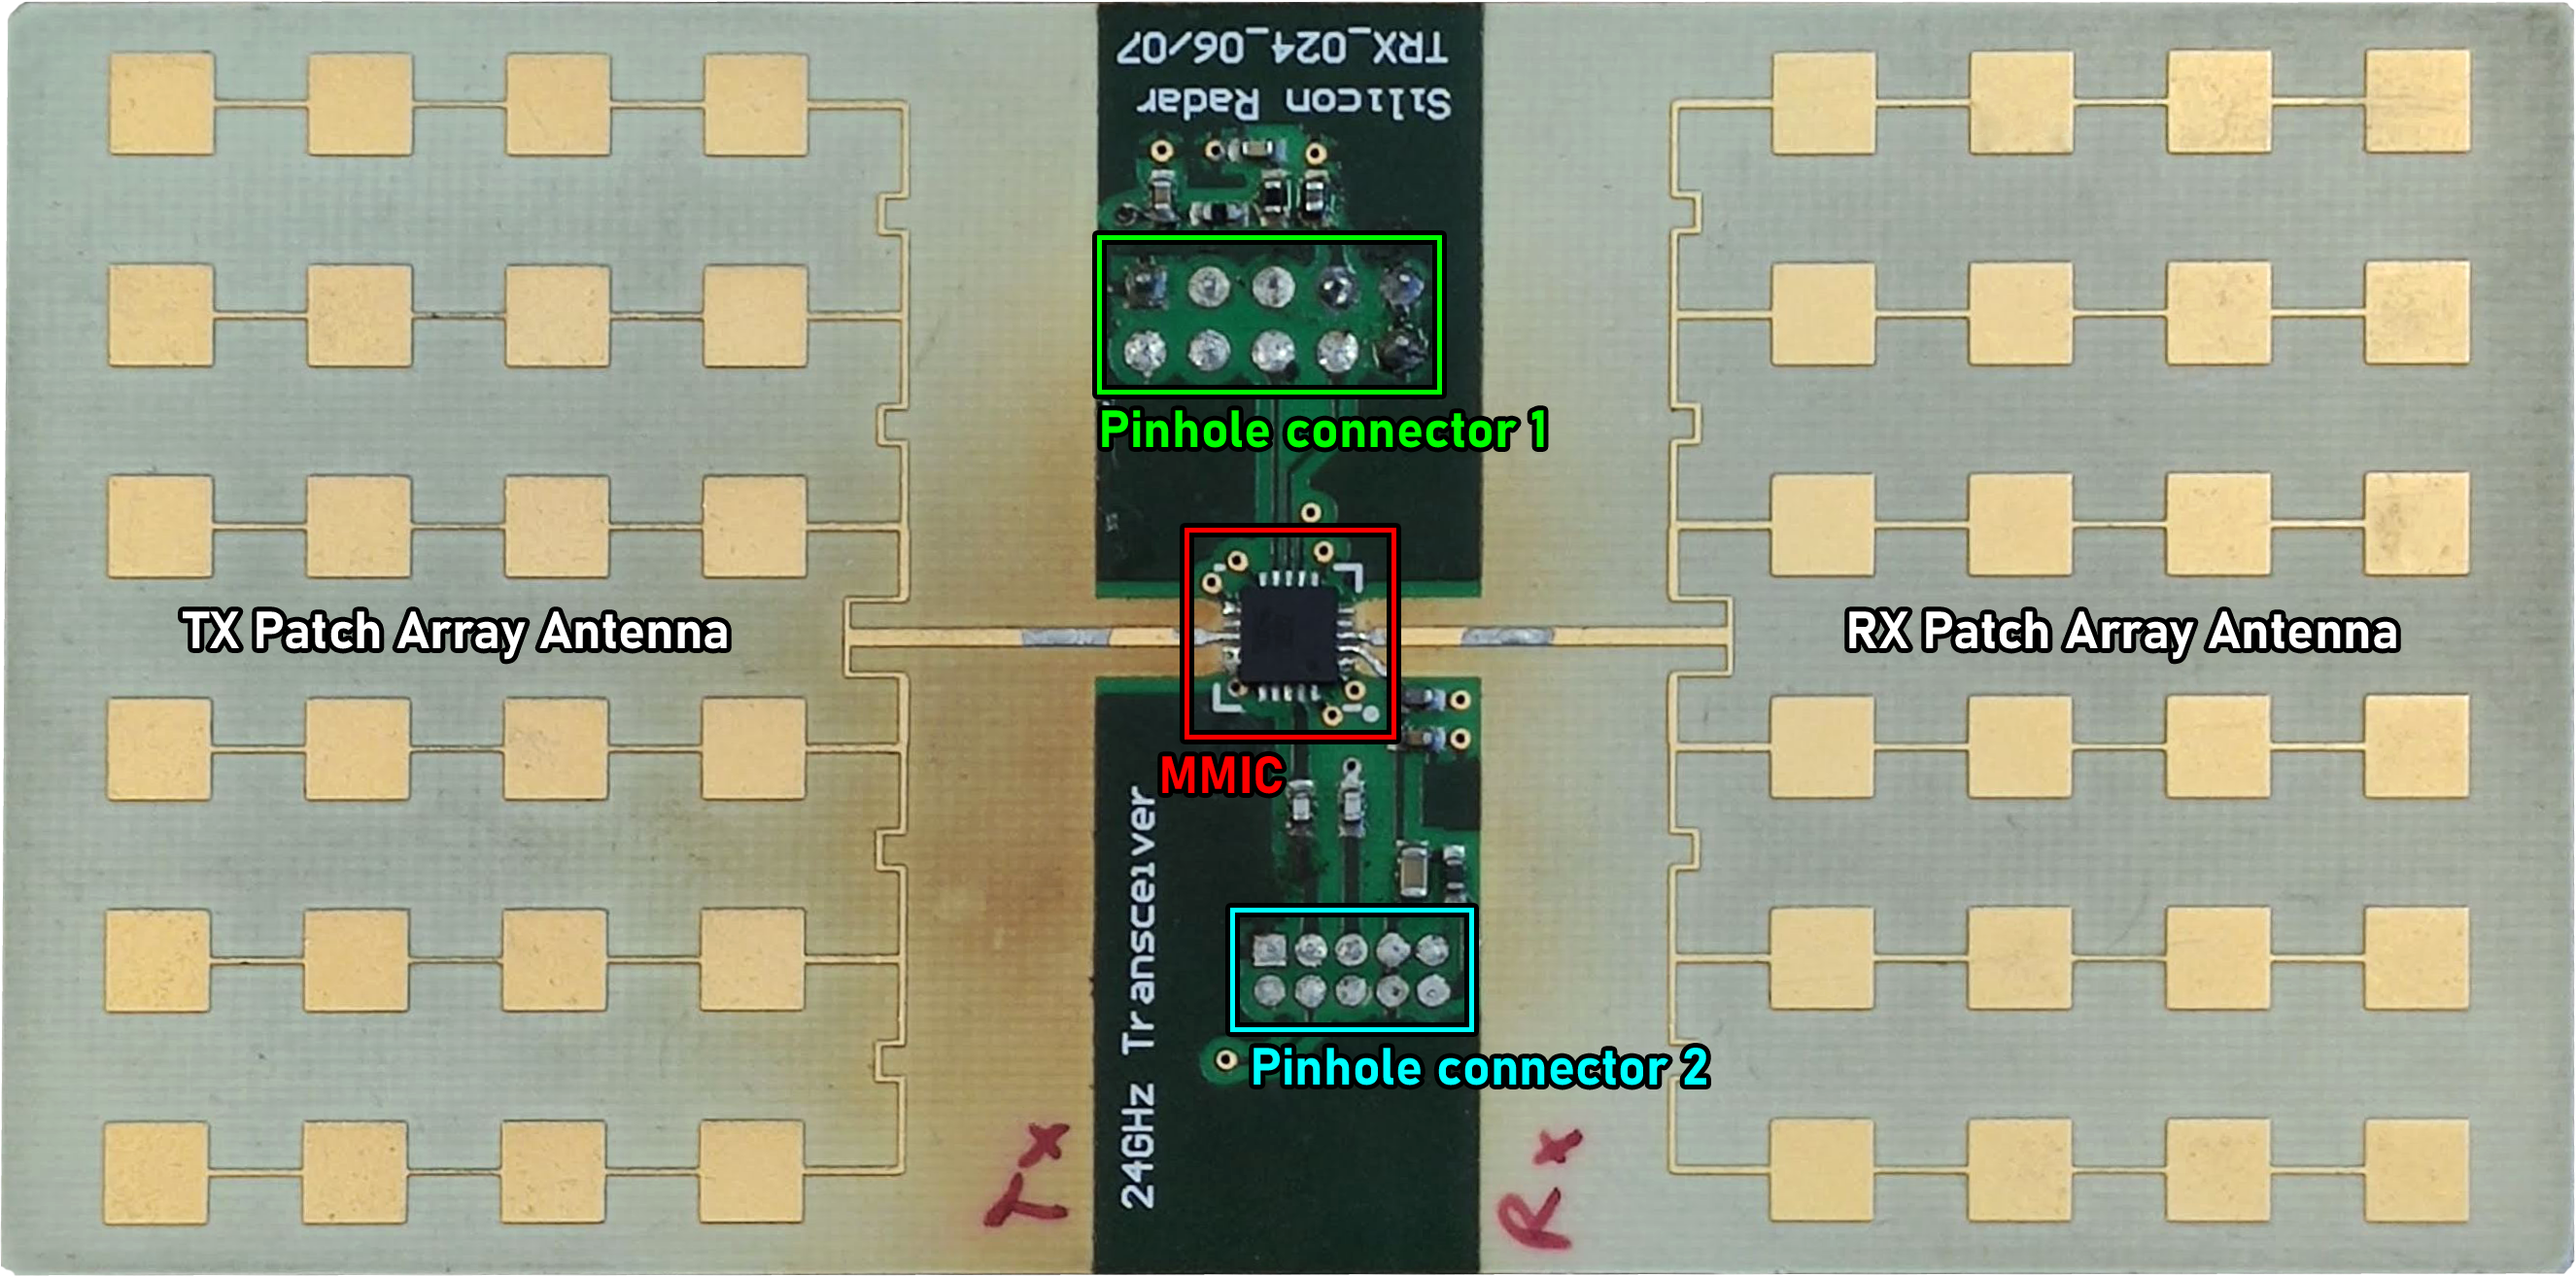
\includegraphics[width=0.8\linewidth]{radar_antenna_mmic.png}
	\caption{Patch antenna and MMIC PCB used in the PCB radar node. The different components are outlined in the image \label{fig:rf_board}}
\end{figure}

This antenna and MMIC module interfaces through the provided pinhole connector with a baseband board.

\subsubsection{Baseband board}

This baseband board follows the general hardware design description outlined in \cref{sec:baseband_general}. The baseband PCB provides the MMIC with the \textit{Vctrl} signal in order to generate the CWLFM ramp signals based on a predefined chirp time and frequency. Additionally, the baseband PCB conditions the IF signals coming from the MMIC.

To generate the correct \textit{Vctrl} values, a phase-frequency detector (PFD) is used. The PFD integrated into the PCB is from Analog Devices, model ADF4159 [REF DS ZZZ]. The device acts as a frequency synthesiser that generates the \textit{Vctrl} signal fed to the MMIC. The PFD is integrated in a phase-locked loop (PLL) architecture described in \cite{Sardinero2022}. A high-level diagram of the PLL architecture for the VCO control voltage generation is shown in \cref{fig:pfd_pll}.

\begin{figure}[ht]
	\centering
	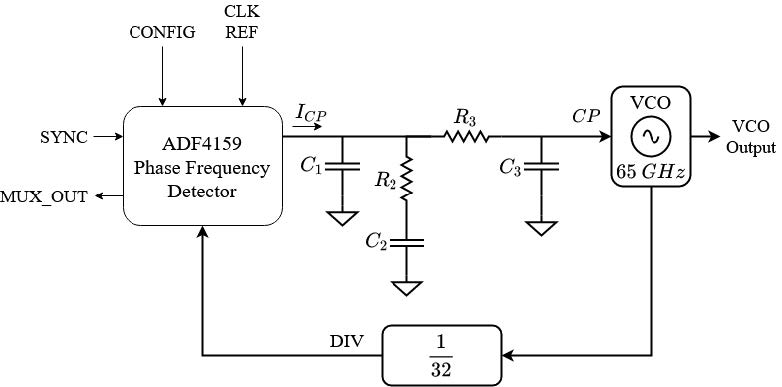
\includegraphics[width=0.9\linewidth]{pfd.jpg}
	\caption{ADF4159 PFD in a PLL architecture with the VCO of the MMIC. The \textit{DIV} signal corresponds to the signal \textit{div\_o} from the MMIC divider (\cref{fig:block_mmic}). The lumped components values are $C_1=\SI{300}{\pico\farad}, R_2=\SI{220}{\ohm}, R_3=\SI{4.7}{\nano\farad},R_3=\SI{470}{\ohm}, C_3=\SI{180}{\pico\farad}$. \cite{Sardinero2022} \label{fig:pfd_pll}}
\end{figure}

Writing to specific registers through SPI communication is used to configure the PFD. A microcontroller unit (MCU) included on the PCB handles SPI communication. This MCU has previously been programmed with the configuration data for the PFD registers. The PFD is configured in accordance with \cite{Sardinero2022}.

Moreover, the baseband PCB is responsible for filtering and conditioning the IF signals output from the MMIC. The raw signals are DC coupled and require a series capacitor to draw the signals to the 0 VDC reference. 


 filters the receiving signals to output intermediate frequency (IF) signals in phase and in quadrature, namely $I_{\mathrm{rad}}$ and $Q_{\mathrm{rad}}$.
\todo[inline]{Describir qué hace exactamente la PCB de banda base, según TFT de Montesano y Nacho S}
En otra subsección
\todo[inline]{Tengo que redactar aquí las características de la señal de IF del documento if\_stage.docx}

\subsection{Conditions of operation}
\change[inline]{Referencia a las condiciones de funcionamiento del radar y explicación de la elección de las condiciones a continuación}
For the purpose of this Bachelor's Thesis, the measurement and operation of the system is carried out under the following conditions:
\begin{equation} \label{eq:if_conditions}
	f_0 = \SI{24}{\giga\hertz} \qquad W = \SI{2}{\giga\hertz} \qquad f_{s\min} = \SI{0.5}{\mega\hertz} \qquad T_c = \SI{529.7}{\micro\second}
\end{equation}

This yields the following maximum operating range ($R_{\max}$):
\begin{align}
	f_s c^2 &= 16 R_{\max}W f_0 \nu_{r\max} \\
	R_{\max} &= \frac{f_s c^2}{16 W f_0 \nu_{r\max}} = \SI{9.917}{\meter}
\end{align}
which is sufficient for an indoor environment of operation requiring around \SI{10}{\meter} distance maximum.

\section{Hardware adaptation and development}
\todo[inline]{Principales desarrollos de la parte MCU e IF (redactar del documento if\_stage.docx), aquí detallar elección de MCU según constraints}
To digitise these signals without losing useful information it is decided to use a microcontroller unit (MCU) with an integrated ADC. The integrated ADC must have a sufficient sampling rate to avoid information loss when sampling as per \cref{eq:nyquist}. In the radar operation conditions, the minimum sampling frequency ($f_{s\min}$) required for the radar signals is given in \cref{eq:if_conditions}. Therefore, for each IF signal ($I_\mathrm{rad}, Q_\mathrm{rad}$) a minimum sampling frequency of $f_{s\min} = \SI{0.5}{\mega\hertz}$ is required.

Moreover, the digitised signals must be transmitted to a receiving device. It is of interest that this transmission is wireless and can be received in a portable device. For that matter, after consideration of multiple wireless communication protocols, Bluetooth Low Energy (BLE) is chosen due to its low-cost and low-power characteristics \cite{Gomez2012}.

The MCU transmits the FFT of each ramp in real-time via the BLE protocol. The MCU features a set of peripherals that allow for adequate sampling, processing and transmission of the signals. 

The chosen MCU that satisfies this conditions is STM32WB15CCU6 from ST Microelectronics which is based on an ARM Cortex-M4 processor \cite{STMicroelectronics2022}. This MCU has an embedded ADC with the following characteristics:
\begin{itemize}
	\item 12-bit resolution, digital range: $[0, 4095]$.
	\item 10 input channels sampled sequentially with a total maximum sampling rate of 2.5 MS/s at 12-bit resolution. When using 2 channels (for $I_\mathrm{rad}$ and $Q_\mathrm{rad}$), each channel is sampled at a maximum of 1.25 MS/s.
	% \item Configurable dynamic voltage range of the inputs: $[0, V_{DDA}]$ where $V_{DDA} \le \SI{3.3}{\volt}$.
\end{itemize}

Additionally, the MCU has an integrated ARM Cortex-M0+ wireless co-processor that handles BLE communication. The BLE communication has the following characteristics:
\begin{itemize}
	\item Maximum theoretical BLE data payload throughput: \SI{1376.2}{\kilo\bit\per\second} \cite{NordicSemiconductor2019,Bluetooth52},  which is not enough to transmit all the raw values from the ADC. Some on-device processing is needed.
	\item Maximum theoretical BLE operating range: \SI{10}{\meter} \cite{Bluetooth52}.
\end{itemize}
\subsection{Signal conditioning}
\unsure[inline]{Tengo que centrarme aquí más en la parte de IF}

The IF stage of the radar amplifies, filters and conditions the intermediate frequency (IF) signals of the radar for the analog to digital (AD) conversion. The radar outputs IF signals in an I and Q format, namely $I_\mathrm{rad}$ and $Q_\mathrm{rad}$. This stage is necessary as the range of $I_\mathrm{rad}, Q_\mathrm{rad}$ does not match the ADC input range. An illustration of this problem is shown in Figure ZZZ.

\todo[inline]{Poner dibujo de señal IF que sale del radar, señal IF que sale del stage}

First, the IF signal is measured and characterised in the ZZZ section. Subsequently, the performance of the ADC is analysed in section ZZZ. Afterwards, the IF stage is designed in section ZZZ, taking into account the input requirements of the ADC and the characteristics of the radar output signal. Finally, the design is laid out on a PCB and measurements and tests are carried out to ensure correct operation in the ZZZ and ZZZ sections.

Two IF signals, $I_\mathrm{rad}$ and $Q_\mathrm{rad}$, are output from the radar. Each signal is composed of a series of beaten frequency ramps. Each cycle interval corresponds to the duration of the radar frequency band sweep as detailed in \cref{sec:radar_sys}. The IF signals captured during one cycle of operation at the conditions in \cref{eq:if_conditions} is shown in Figure ZZZ. It is shown that the amplitude of the IF signals at the center of the selected interval is remarkably higher than the amplitude of the IF signals at the edges of the selected interval. This is a consequence of using narrow-band antennas: the amplitude of the beat signal is higher when the antenna is resonant.

The measurement of the IF signals has been carried out in an Agilent Infiinium 54832B oscilloscope with inputs loaded with \SI{50}{\ohm}.

The IF signals of the radar $I_\mathrm{rad},Q_\mathrm{rad}$ have the following characteristics:
\todo[inline]{características del if\_signal\_excursion.docx}.

\begin{figure}[ht]
	\centering
	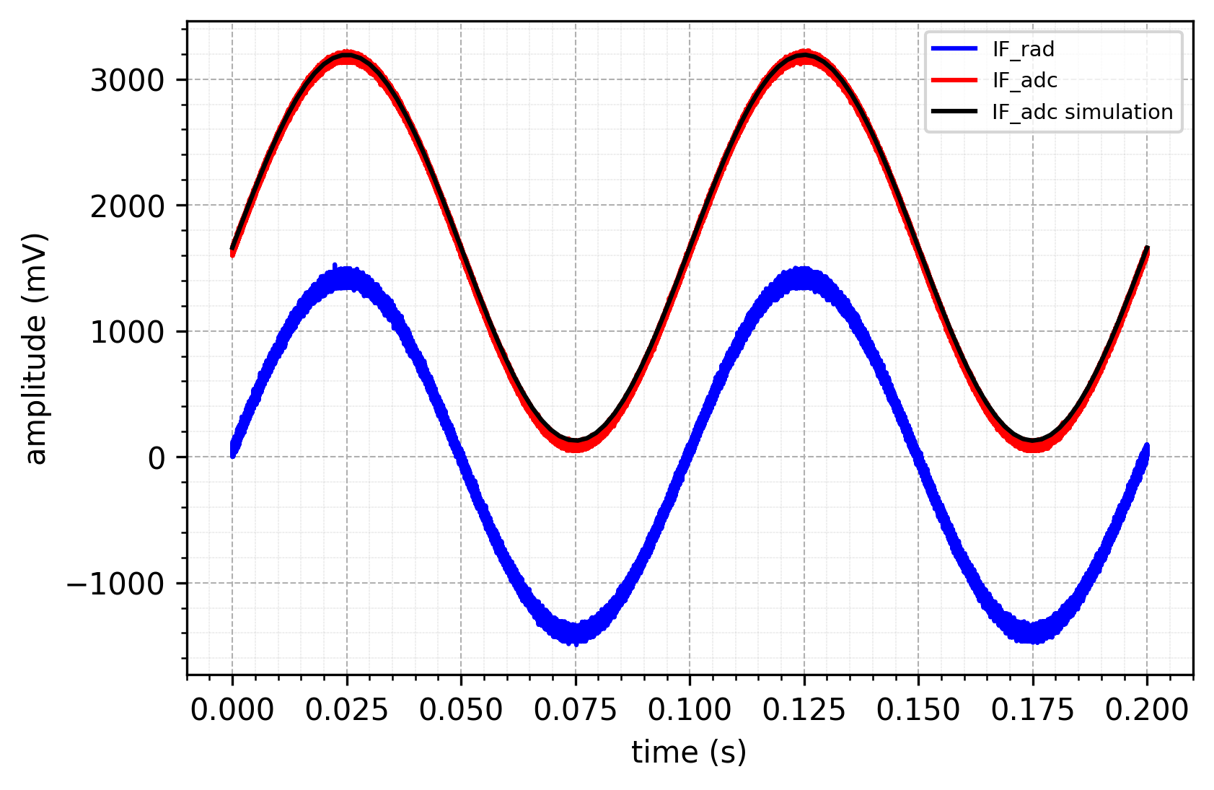
\includegraphics[width=0.7\linewidth]{sucio_graficos/if/10hz.png}
	\caption{Sin 10 Hz}
	\label{fig:moduloaprox50cmplancha}
\end{figure}
\begin{figure}[ht]
	\centering
	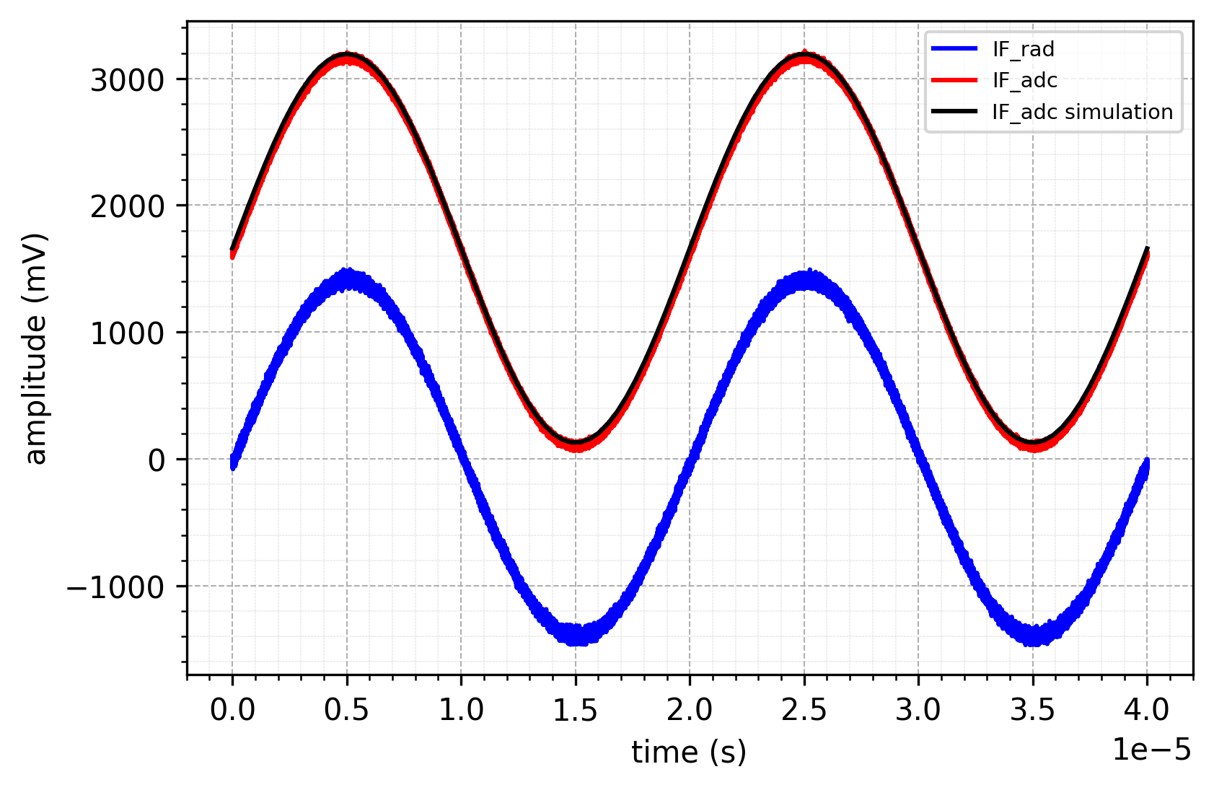
\includegraphics[width=0.7\linewidth]{sucio_graficos/if/50khz.png}
	\caption{Sin 50 kHz}
	\label{fig:moduloaprox50cmplancha}
\end{figure}
\begin{figure}[ht]
	\centering
	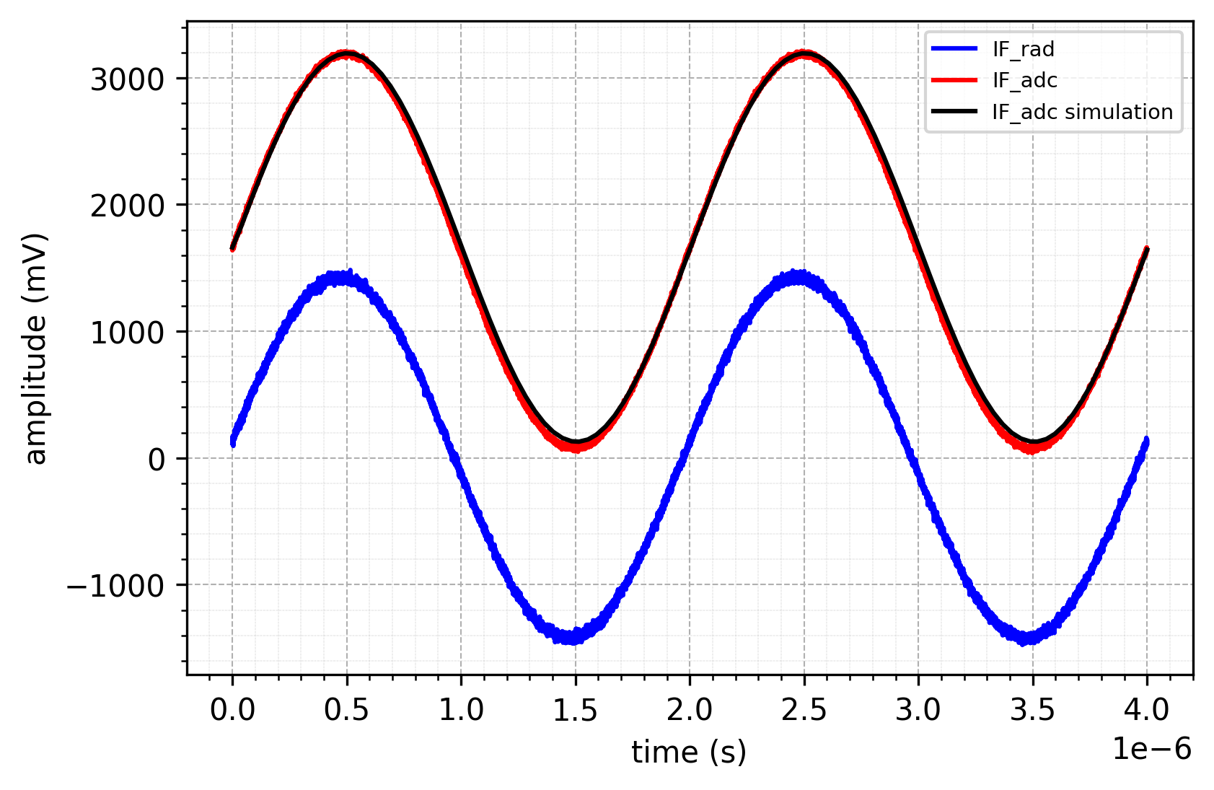
\includegraphics[width=0.7\linewidth]{sucio_graficos/if/500khz.png}
	\caption{Sin 500 kHz}
	\label{fig:moduloaprox50cmplancha}
\end{figure}
\begin{figure}[ht]
	\centering
	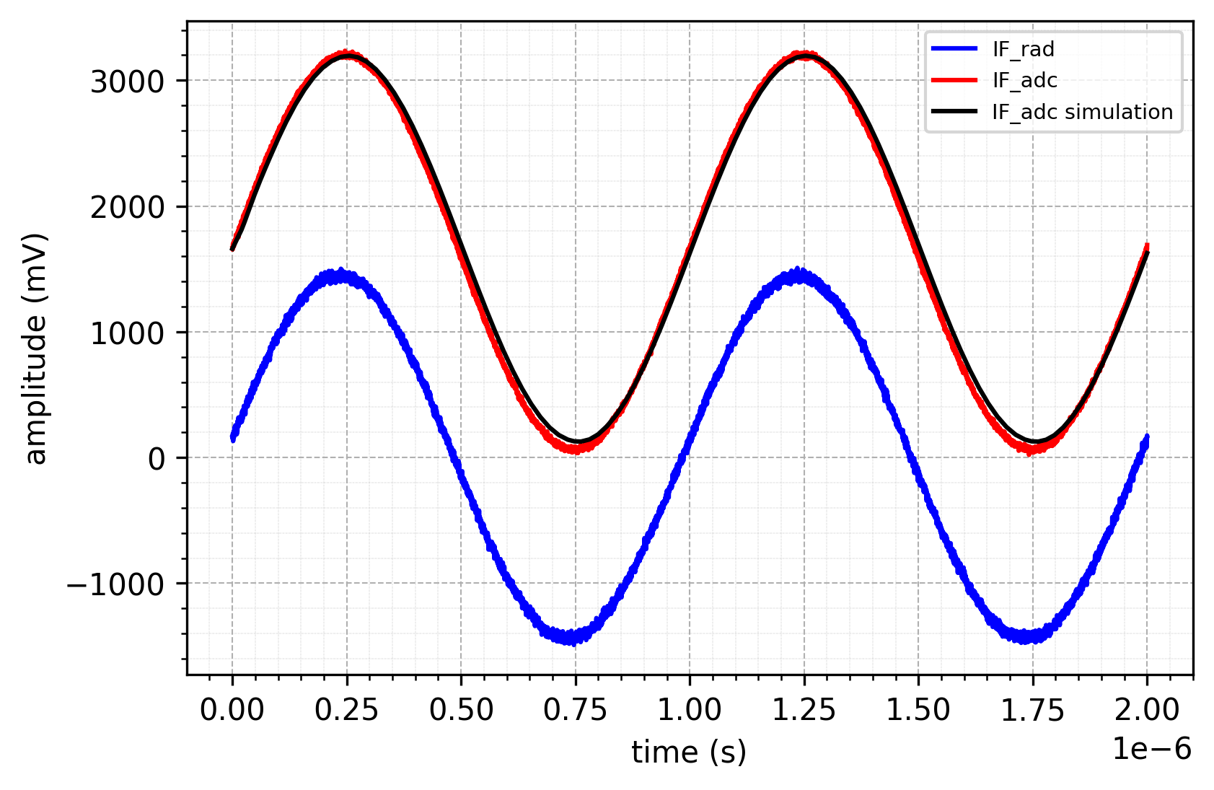
\includegraphics[width=0.7\linewidth]{sucio_graficos/if/1mhz.png}
	\caption{Sin 1 MHz}
	\label{fig:moduloaprox50cmplancha}
\end{figure}

\subsection{Digital signal processing}
\unsure[inline]{Tengo que centrarme aquí más en la parte del pipeline de procesado (tengo que redactar microdoppler mode junto con la documentación del sistema), sacar esto del dsp\_chain.md}
\subsection{Wireless communication}
\unsure[inline]{Tengo que centrarme aquí más en la parte del pipeline de procesado (tengo que redactar microdoppler mode junto con la documentación del sistema), tramas, etc, hablar de protocolos y comparación de protocolos wireless (ble al final mejor por compatibilidad, y consumo energético)}

\begin{figure}[ht]
	\centering
	\subfloat[Bottom view]{\includegraphics[width=0.5\linewidth]{img/radar_pcb_bot.png} \label{fig_cwlfm_ramps_freq}}
	\subfloat[Top view]{\includegraphics[width=0.49\linewidth]{img/radar_pcb_top.png} \label{fig_cwlfm_diff}}
	\todo[inline]{TODO: Change this layout for a diagram of necessary parts of a baseband board, leave this layout for our implementation}
	\caption{Views of a manufactured PCB featuring an example layout of the baseband stage reference design \label{fig:bb_board}}
\end{figure}

\chapter{Characterisation of the radar node}
\section{IF stage characterisation}
Aquí van las medidas del powerpoint redactadas:
\begin{itemize}
	\item Simulaciones de señales IF en el rango de tensiones y frecuencias
	\item Medidas de señales IF en el rango de tensiones y frecuencias
	\item Respuesta en frecuencia, simulación del TINA: bode\_plot.tiff y explicar que cubre el ancho de banda de las señales en banda base.
	\item Respuesta en frecuencia, medidas bode manual: del bodeplot del matplotlib y explicar que cubre el ancho de banda de las señales en banda base, y que es similar a la simulación
\end{itemize}

\section{ADC characterisation}
Aquí van las medidas del powerpoint redactadas, sobre el ADC:
\begin{itemize}
	\item Ruido de fondo del ADC. En tensiones y en dB.
	\item Simulación de adquisición del ADC del MCU: medidas adc\_sampling.staertsim3, sacar esto a .csv y poner plots
	\item Medidas de adquisición del ADC del MCU: medidas adc\_iq\_raw.hex de la memoria del micro, poner y explicar los gráficos del python
\end{itemize}
\begin{figure}[ht]
	\centering
	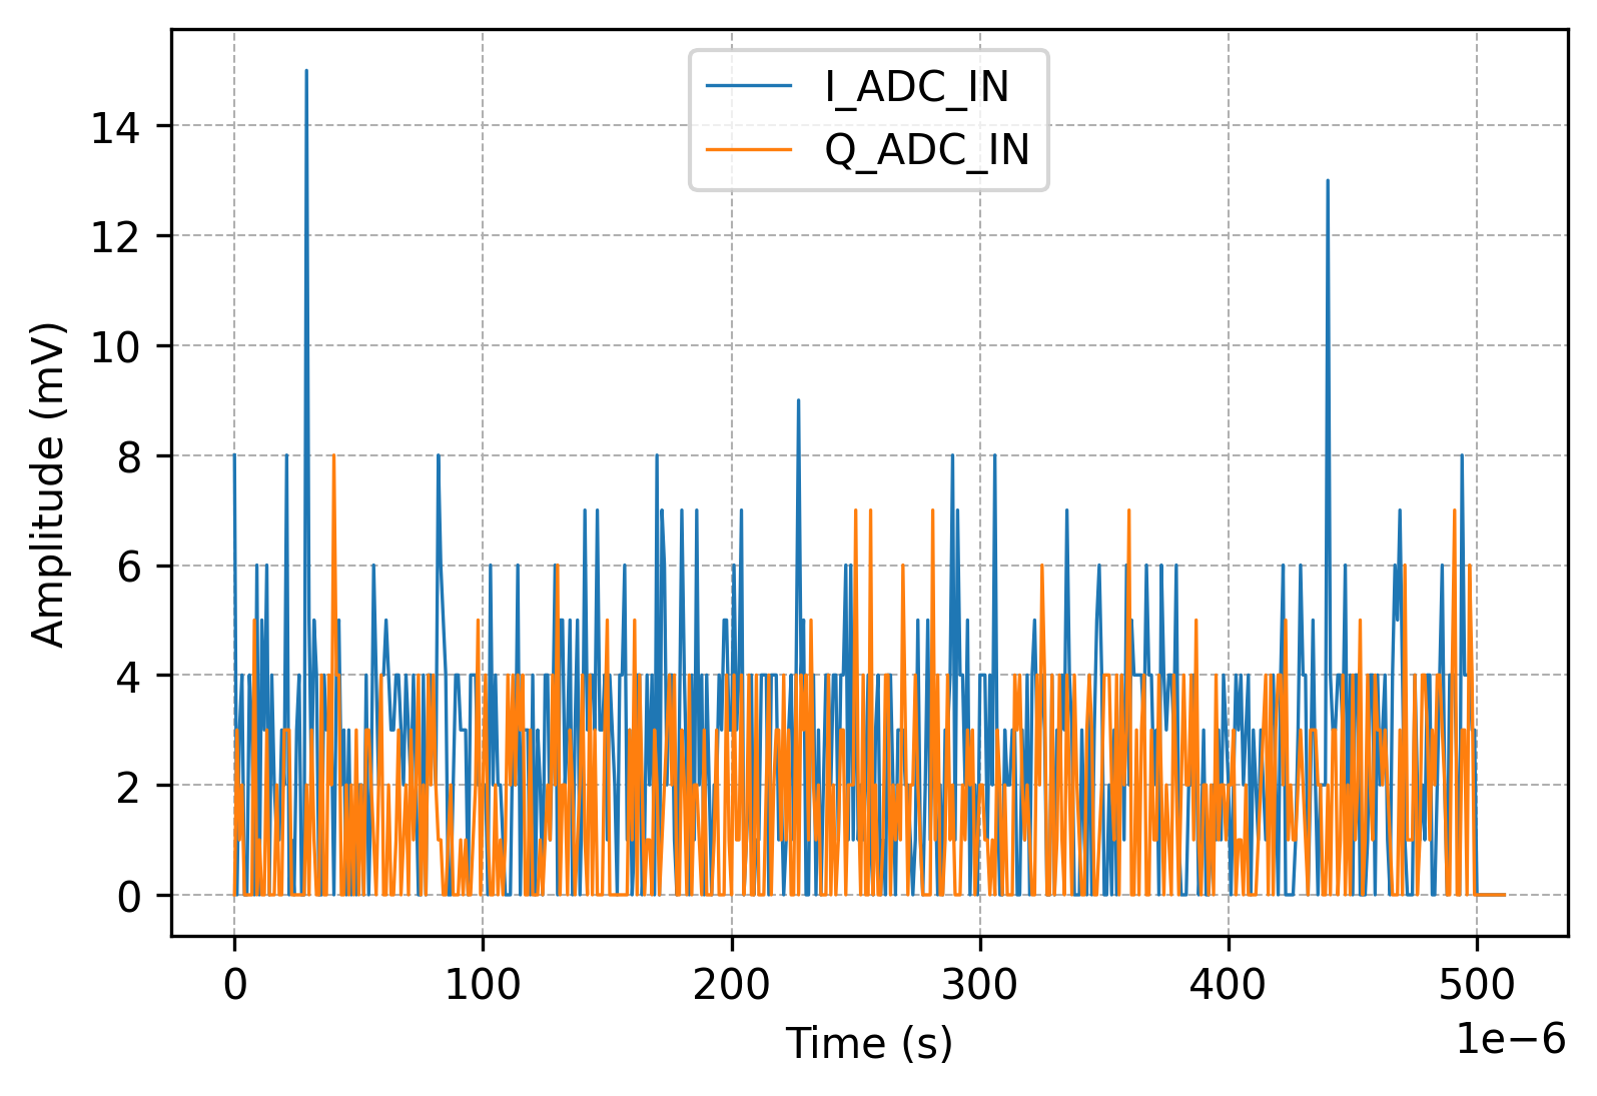
\includegraphics[width=0.7\linewidth]{sucio_graficos/adc/nf_mv.png}
	\caption{Noise Floor in mV}
	\label{fig:moduloaprox50cmplancha}
\end{figure}
\begin{figure}[ht]
	\centering
	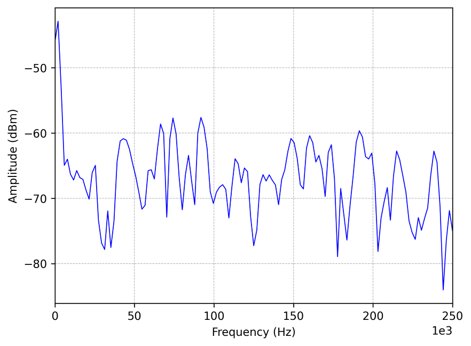
\includegraphics[width=0.7\linewidth]{sucio_graficos/adc/nf_dbm.png}
	\caption{Noise Floor in dBm}
	\label{fig:moduloaprox50cmplancha}
\end{figure}
\section{DSP Characterisation}
Aquí van las medidas del python redactadas, sobre el DSP pipeline:
\begin{itemize}
	\item Conversión a coma fija, explicar gráfico del error: conv\_q15\_error.eps y concluir que el error es menor del 1\% del rango de entrada del ADC, por lo que guay.
	\item Conversión a coma fija, ejemplos de medidas reales, del memdump adc\_iq\_q15.hex
\end{itemize}
\section{Wireless stack Characterisation}
Aquí van las medidas del python redactadas, sobre el BLE:
\begin{itemize}
	\item Caracterización binary throughput
	\item Caracterización BER
	\item Caracterización Ramp Lost Ratio to Distance
\end{itemize}
\begin{figure}[ht]
	\centering
	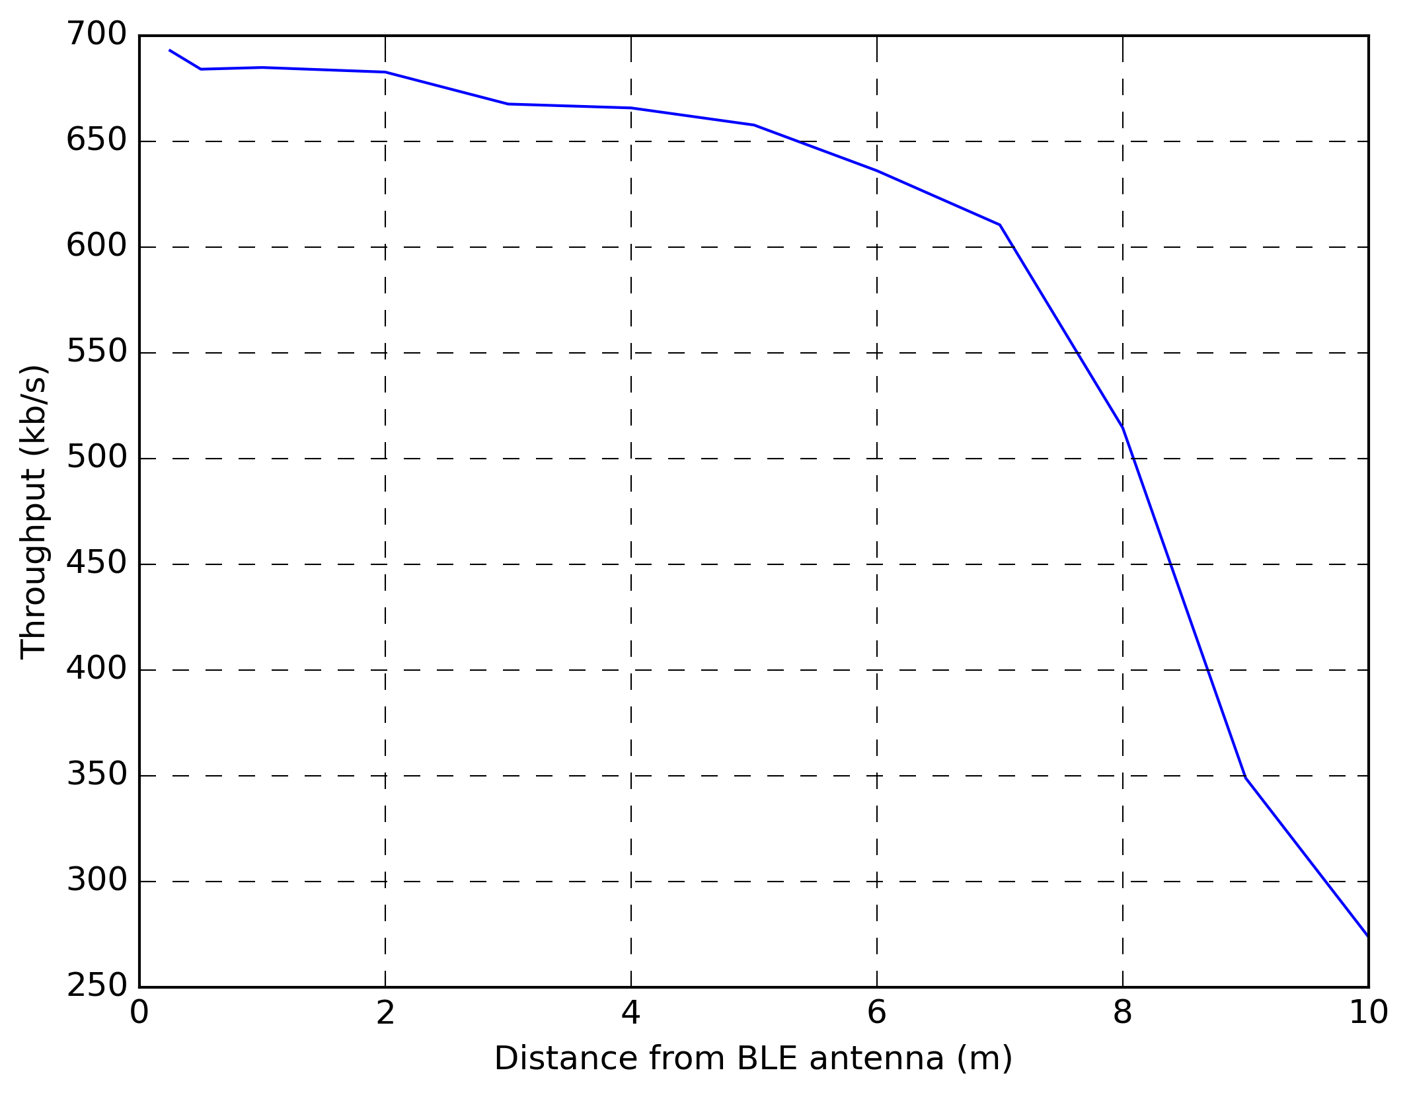
\includegraphics[width=0.7\linewidth]{sucio_graficos/ble/throughput.png}
	\caption{BLE Throughput vs distance}
	\label{fig:moduloaprox50cmplancha}
\end{figure}
\begin{figure}[ht]
	\centering
	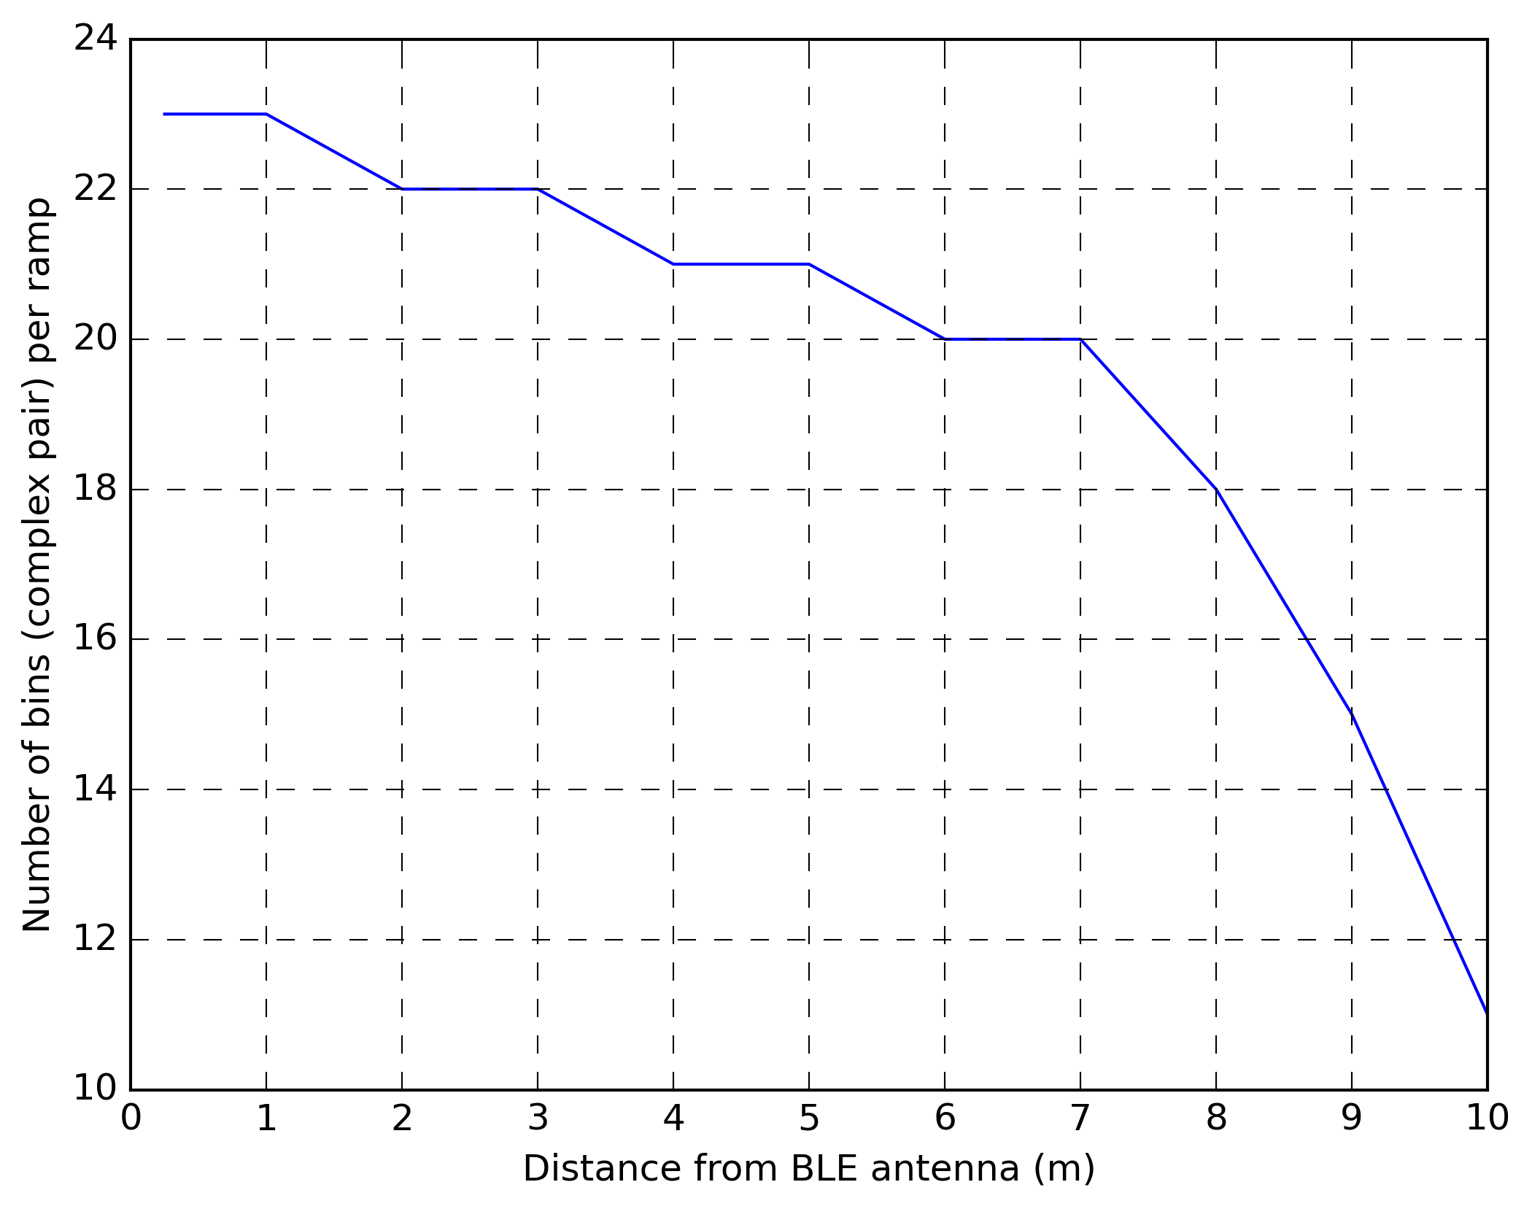
\includegraphics[width=0.7\linewidth]{sucio_graficos/ble/bins_per_ramp.png}
	\caption{Maximum transmitted bins per ramp without ramp loss vs distance}
	\label{fig:moduloaprox50cmplancha}
\end{figure}
\begin{figure}[ht]
	\centering
	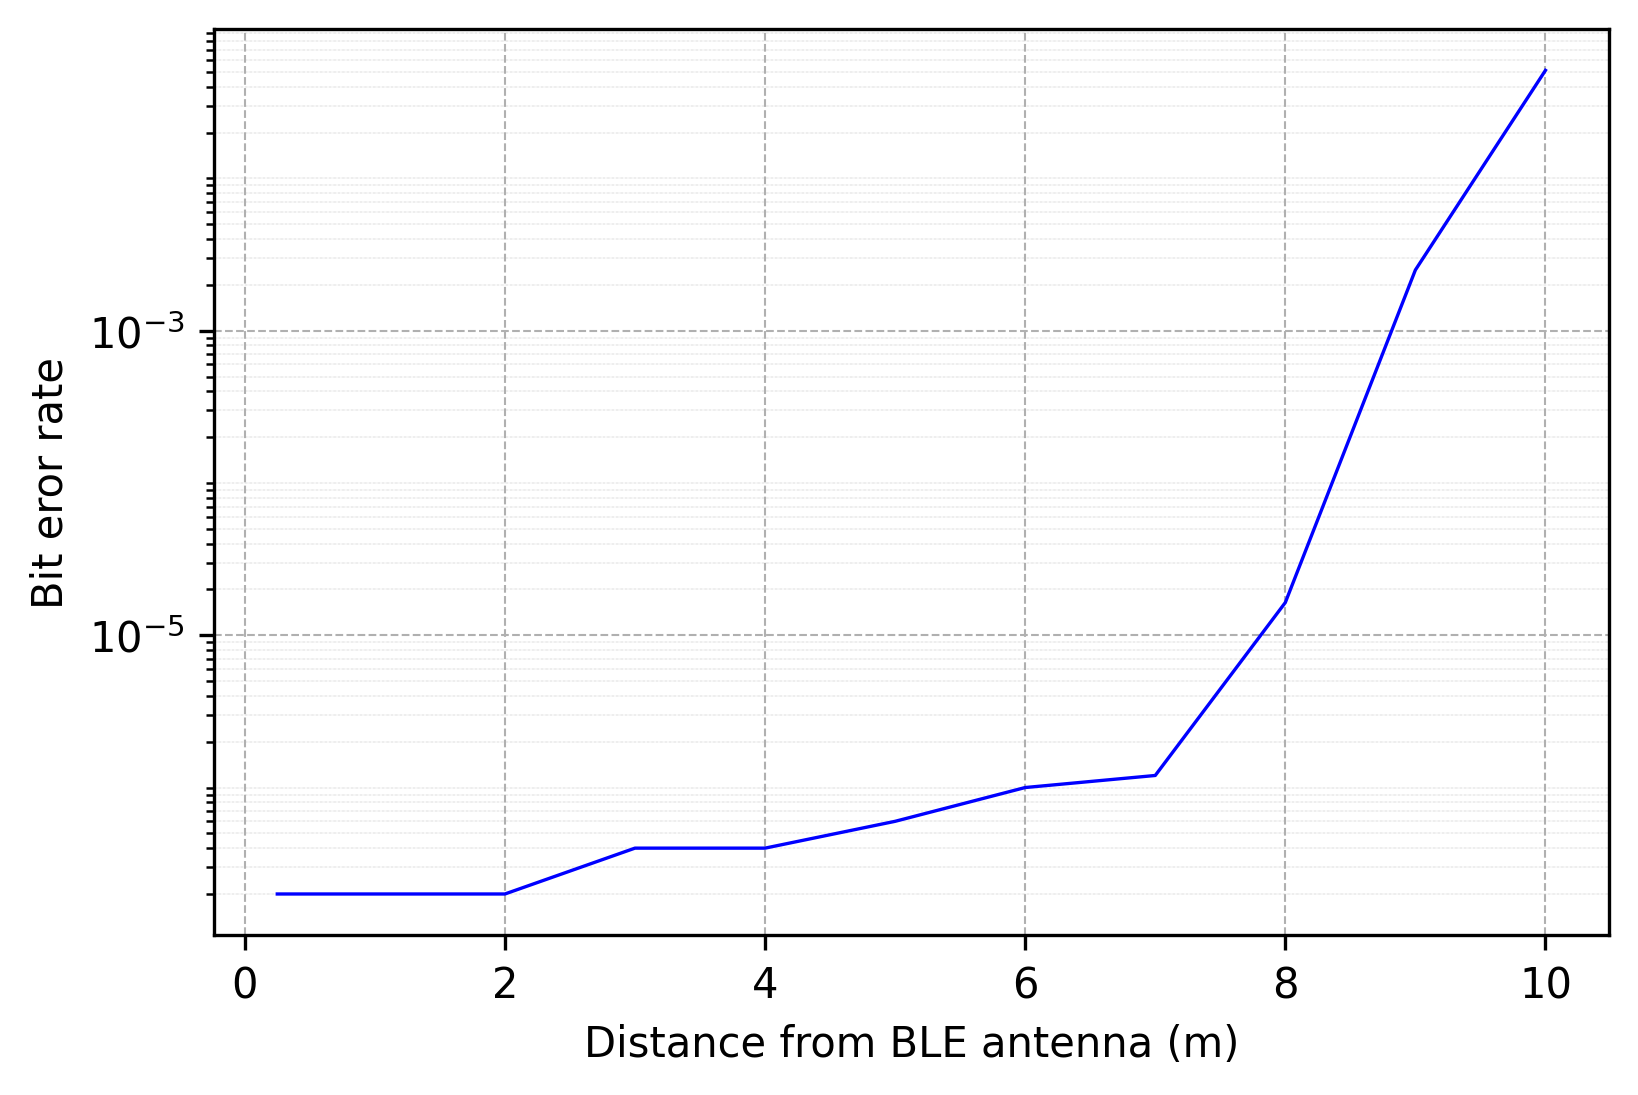
\includegraphics[width=0.7\linewidth]{sucio_graficos/ble/ber.png}
	\caption{Bit error ratio (BER) of the wireless communication link (revisar ZZZ)}
	\label{fig:moduloaprox50cmplancha}
\end{figure}
\begin{figure}[ht]
	\centering
	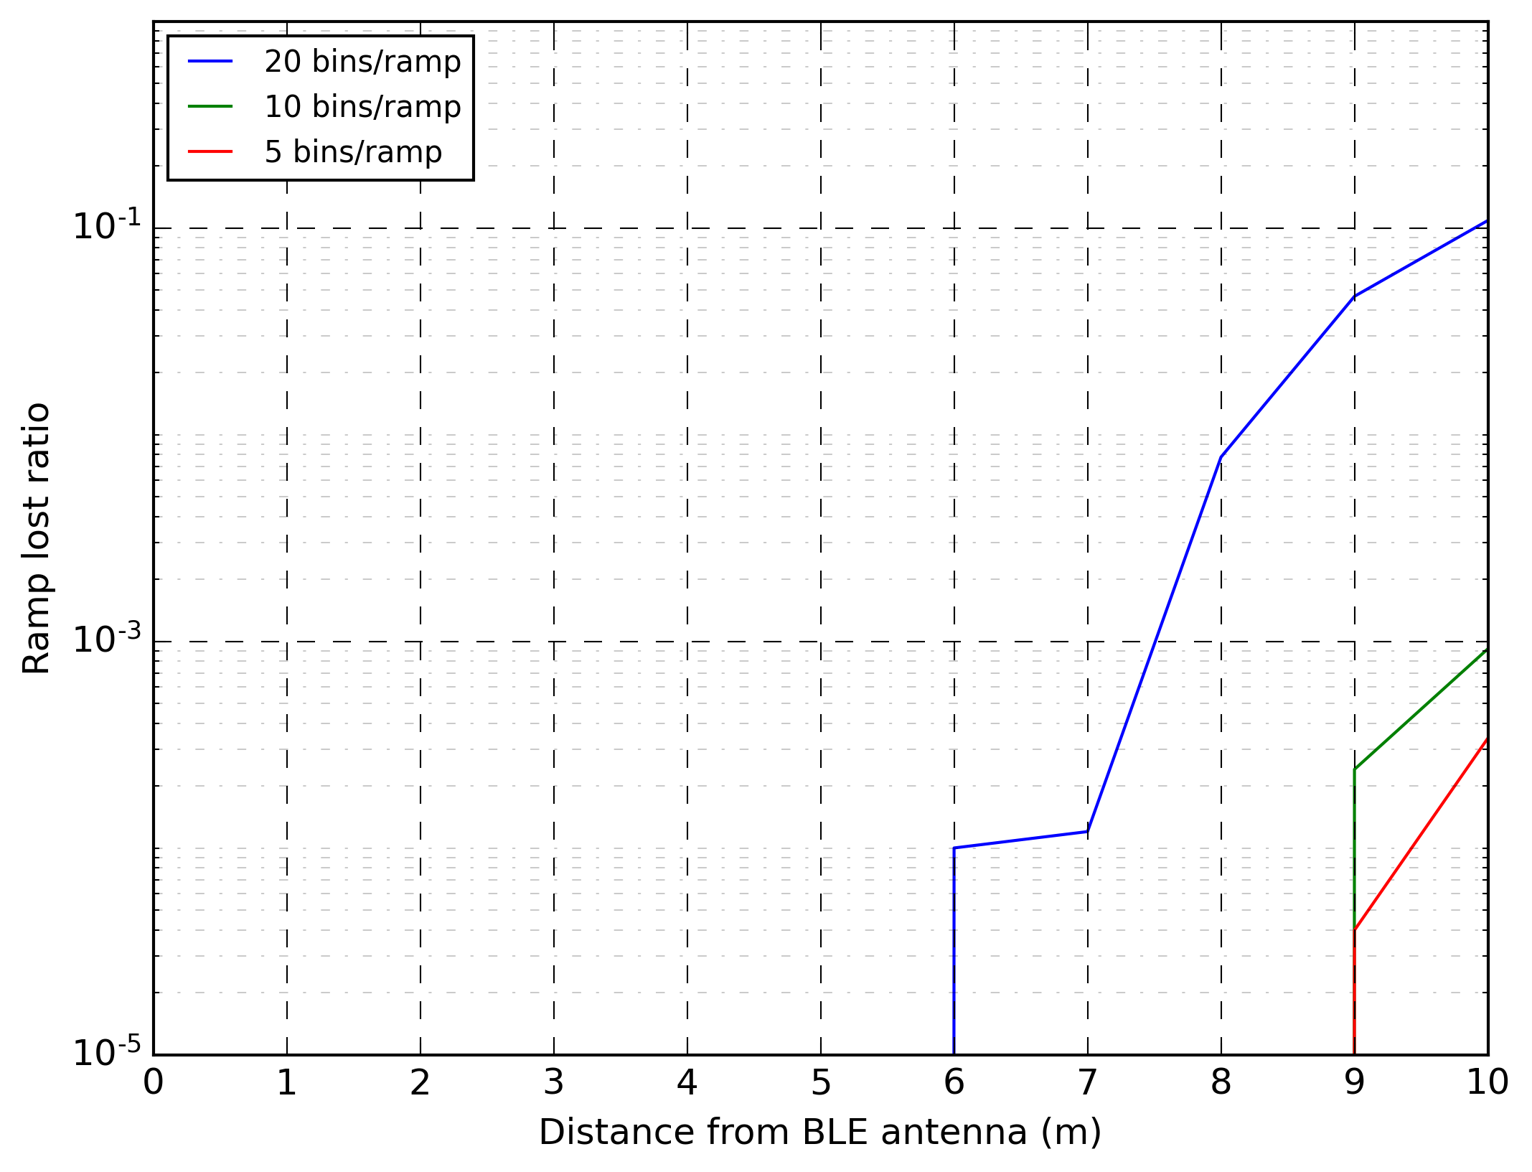
\includegraphics[width=0.7\linewidth]{sucio_graficos/ble/rlr.png}
	\caption{Ramp lost ratio vs distance}
	\label{fig:moduloaprox50cmplancha}
\end{figure}

\unsure[inline]{Medida de la ecuación radar}
% el problema requiere el uso de radares cwlfm que son compactos, eficientes en coste y de bajo consumo

% establecer las condiciones de operación para las pruebas, requisitos radar/comunicaciones, hablar de anchos de banda, bitrate, etc. caracterización de las señales de frecuencia intermedia.

% adaptación hardware, creación sistema hardware, 
%		hablar de mcu, seleccion mcu debido a qué criterios. hablar del adc del mcu
%		diseño de etapa if para adaptar el nivel de la señal.
%		desarrollo del pipeline de procesado digital de señal
%		desarrollo del pipeline de transmisión bluetooth
%		desarrollo de aplicación pc

% otro chapter
%		caracterización de las distintas partes

